\chapter{Space Reduction Approach}
\label{ch:approach}

In this chapter, I discuss the adopted approach to substantially mitigates the space inefficiency of Hypertrie.  
The technique relies mainly on compressing a Hypertire path with specific characteristics. 
Worth mentioning that the approach does not neglect the other attempts already realized to minimize Hypertrie's memory footprint. 
In contrast, it could be considered an added feature that further contributes to the space reduction of the overall Hypertrie data structure. \\

This part of the work delivers motivation to the approach. Afterward, an illustration of the new Hypertrie internal nodes' design needed to realize the solution is delivered. The chapter ends with a presentation of the cor algorithms that define the behaviors of the newly designed Hypertrie. 


\section{Hypertrie Memory Utilization}
\label{sec:hypertrie_memory_utilization}
Despite its operational efficiency, Hypertrie performance comes not without a trade-off. 
Since Hypertrie is a special kind of a Trie data structure, it inherits some of the fundamental problems of  Tries. 
One of these problems is the excessive space utilization in a worst-case scenario \cite{Brass:2008:ADS:1434862}.  \\

The current design and implementation of Hypertrie \cite{tentris2020}, however, mitigates the space inefficiency characteristic in two ways. 
First, each partial function $c^{(h)}_i$ (Def. \ref{def:bht}) in each hypertrie node $h$ is realized using a custom sparse hash table $HT$ instead of arrays or linked lists to store the key parts. 
By using hash table, Hypertrie's nodes only stores keys that form prefixes to already existed paths. 
In contrast, arrays utilization in normal Tries considers the whole alphabet set in each node with many array entries store pointers that refer to null (Sec. \ref{sec:trie}).  \\

The adoption of hash tables in Hypertrie also delivers extra performance as looking up keys is nearly constant compared to linked list search where it has a linear computational complexity $O(n)$. 
The other attempt to reduce the overall space requirement is to store equal nodes (Sub-hypertrie) only once by making use of the associativity characteristic of the slicing operations in tensors (Sec. \ref{sec:tensor_algebra}). That is, hypertrie takes advantage of that fact that the slicing order relative to the root node has no influence when slices are chained. Example: $T[k_0, k_1, ....] = (T[k_0, :, ....])[k_1, ....] = (T[:, k_1, ....])[k_0, ....].$ \\

By exploiting the equivalent slicing concept and store equal sub-hypertrie nodes only once, it is proved that the upper storage bound of hypertrie $h \in H(d)$ is $\vartheta(2^{d-1}. d . z(h))$, where $z(h)$ is the number of non-zero entries \cite{tentris2020}. Since, hypertrie realizes an RDF tensor, then $d=3$. Thus, the upper storage bound is $\vartheta(12 . z(h))$.
\vspace{0.5cm}

\section{Space Reduction Solution}
Despite the previously mentioned attempts to minimize the size of Hypertrie (Sec. \ref{sec:hypertrie_memory_utilization}), the excessive memory utilization is still a bottleneck. The case can be witnessed in practice when the set of RDF triples needed to be indexed by hypertrie increases in size with less overlapping between its triples. As a result, a set of nodes, including the root node, will store edges to children with single entry for a particular dimension. Nevertheless, we still need to utilize a space to host a pointer to that child node. This results in a space redundancy issue \cite{PATRICIA}. 

\begin{example}
\label{ex:space_problem}
Back to the example depicted in figure \ref{fig:rdf_hypertrie}:
\begin{enumerate}
	\item The inner node labeled with \verb|<4, :, :>| contains an edge = 3 at position 1 that maps to leaf node with a single entry. 
	\item Another example in the same structure is the root node $r$ along with its child $h = c_0^{(r)}(5)$. It is noticeable that  $h$ also map its edges to single-element lead nodes.
\end{enumerate}

\end{example}

Inspired by PATRICIA \cite{PATRICIA}, the redundancy problem mentioned above can be eliminated by recursively storing a single-element children into their parent nodes resulting in a \textit{path compression}. In other words, we compress the hypertrie branches by storing \textit{key suffixes} into their parent node at the key part from which the suffix was branched. Back to the example \ref{ex:space_problem}, the leaf node labeled with \verb|<4, :, 3>| can be compacted along with its parent edge in its parent node \verb|<4, :, :>| at the edge 3. Similarly, the leaf nodes \verb|<5, 6, :>| and \verb|<5, :, 7>| can be stored into their parent node \verb|<5, :, :>| at the respective edges. However, the parent node itself represents a single sub key, hence it can be compacted into the root node at edges = 5 in position 0. \\

Applying the path compression approach this way will introduce a modified version of hypertrie, a \textit{compressed hypertrie}. Edges that map to key suffixes stored in parent nodes are termed as \textit{compressed edges}. 
Figure \ref{fig:rdf_compressed_hypertrie} depicts a compressed hypertrie variant that stores the RDF graph $g$ in table \ref{tab:rdf_graph_example}.
when the path compression technique is applied. It is noticeable that many keys stored in the second level nodes (depth=2) do not need to be branched further to point to other nodes in the third level. 
As a result, the tree height is cut down, and a substantial amount of memory is saved by storing objects in-place instead of allocating extra space to store pointers to children. 

\begin{sidewaysfigure}[htbp]
	\centering
	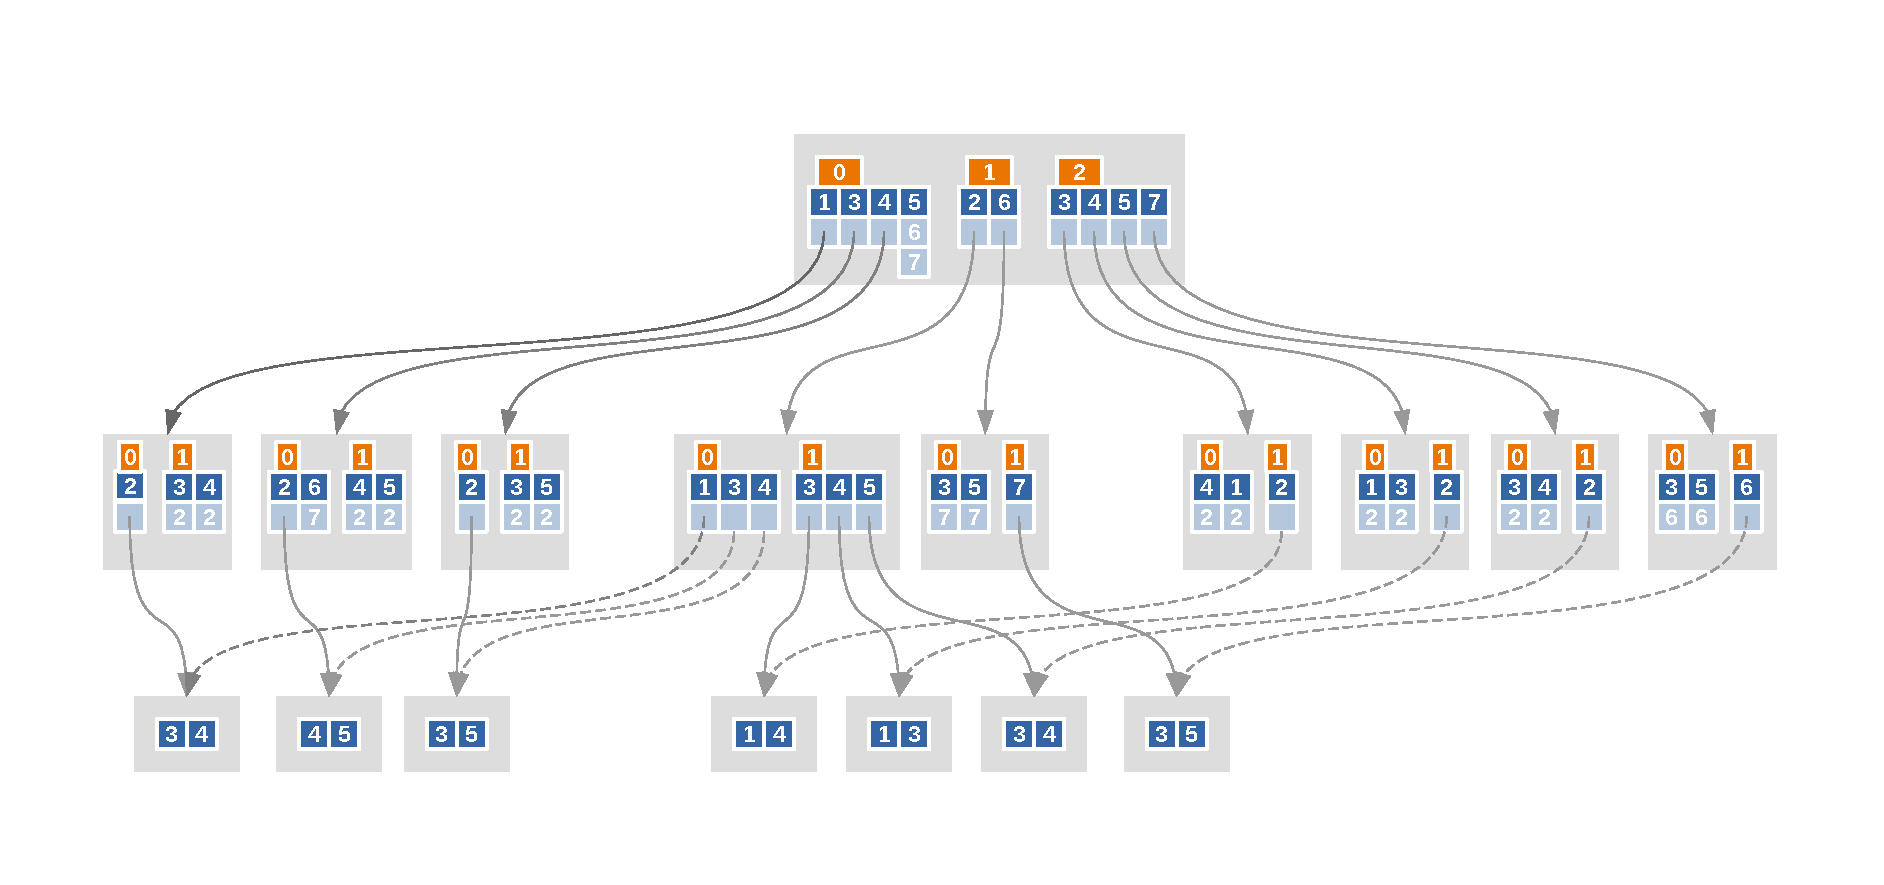
\includegraphics[scale=0.74]{figures/chapter4/compressedBHT}
	\caption{Storing RDF in space-efficient Hypertrie (Compressed Hypertrie).}
	\label{fig:rdf_compressed_hypertrie}
\end{sidewaysfigure}


\section{Compressed Hypertrie Nodes}
\label{sec:compressed_nodes_representation}
In order to achieve path compression in Hypertrie, fundamental design changes need to take place. By that, we can enable the node to store the entire key suffix.
As the size of key suffixes varies depending on the depth of the parent node, each group of Hypertrie nodes at certain depth will have their own internal node representation. In details, each hypertrie node of depth $d$ should realize a \textit{container} concept of size $d-1$ for every compressed path stored in it. On the other hand, compressed hypertrie nodes should be \textit{adaptive} to change. As the hypertrie state changes, for example by adding a new key, holding a compressed key path at certain edge may no longer be valid. The node at that particular edge mush be branched down to child nodes. \\

From programming point of view, the redesign of Hypertrie nodes' structures is low level. Thanks to C++17 template meta-programming features, we could separate the compressed nodes realization from the Hypertrie data structure interface. By that, we can still insure a smooth integrity of Hypertrie with other components in Tentris system. In this section, I delve into the internal design of each type of compressed hypertrie nodes and discuss the concept of virtual node that enable slicing in the compressed mode. \\
\begin{remark}
The following sections make use of all the terminologies, definitions, and conventions defined in section \ref{sec:preliminaries:tentris} that refer to various aspects of tensors and trie (including hypertrie).
\end{remark}

\begin{remark}
	The term $H(d)$ in the following sections will refer to the set of all nodes of depth $d$ in the compressed version of hypertrie, not the original hypertrie.
\end{remark}


\subsection{Internal Node Representations}
\label{ch:approach_node_structure}
This section summarizes the design decision of compressed hypertrie nodes. A major step to implement the path compression approach is to the container concept for each node type\footnote{Leaf nodes are not considered.} (Sec. \ref{sec:compressed_nodes_representation}).
As a result, each inner node should still be able to expand at certain edges to sub Hypertrie nodes while maintaining a compressed key path stored in containers bounded to other edges (compressed edges). \\

The compressed key path container implementation varies depending on the node depth. Since Hypertrie's internal nodes can be either a root node or depth two nodes, we can distinguish two variants of internal node representations: \\

\subsubsection{Depth 3 Node (root node)} 
%As the Hypertrie has a predefined fixed depth $d = 3 $, There exists a single root node. 
In addition to the set of edges (hash tables) $HT_{p}$ for each position $p \in P = \{0, 1, 2\}$, the root node $r \in H(d = 3)$ additionally holds another array of hash tables $CommHT_{p}$ that maps key parts $k_{j}$ to static arrays $arr_{j}$ of the size $d -1 = 2$. 
Each array will serve as the container for the key path prefixed by the associated key part $k_{j}$ at the corresponding position $p$ as depicted in Fig. \ref{fig:compressed_depth_3_node}. 
In this context, the key part $k_{j}$ stored in $CommHT_{p}$ represent a compressed edge. Clearly, a key part at a particular position $p$ can either represents a compressed or non-compressed edge at a time, so it exists in either $HT_{p}$ or $CommHT_{p}$. 
The remaining key path $k_{S} = <k_{1}, k_{2}>$ associated with each compressed edge $k_{j}$ holds the key part chain ordered by their presence in the key. \\

Worth to mention that the key path associated with each compressed edge still represents a $2D$ sparse tensor $S$ that results from slicing tensor $T$ represented by the root node at position $p$ with key part $k_{j}$. The resultant tensor $S$ has a single entry $<k_{1}, k_{2}>$ that evaluates to $1$. 
As a result, it is important to maintain the order of the elements in the compressed path $arr_{j}$ as each key $arr[i]$ represents the single edge at position $i$ in $S$ whose child is the other array entry. \\

\subsubsection{Depth 2 Node} Internal nodes $h_2 \in H(2)$ realize the static container concept associated with compressed edges differently than for the root node. 
Considering the number of internal nodes, it becomes unfeasible to assign extra set of hash tables for each node that serve as containers for key part chains. \\

To implement the container concept, the design of depth 2 nodes exploits the fact that key suffixes for edges comprise a single key part.
Hence, we could reuse the space already booked to store the pointers to child nodes (leafs) to hold the suffixed key part.
For the pointer $ptr_{j}$ associated with the edge $k_{j}$ to serve the purpose of either pointing to a child node or holding an integer value, we make it a tagged pointer (Sec. \ref{sec:preliminaries:pointertagging}). \\

Consequently, pointers to children that corresponds to edges $k_{j}$ in $h_2$ are denoted by $ptr_{j} = (value, tag)$. Such pointers carry two pieces of information. (1) A $value$ is the actual payload of bits, which can be viewed as either a memory address or a raw integer value depending on the tag value. (2) A $tag$ is the value held in the least significant bits (LSB) indicating whether the associated edge $k_{j}$ is compressed or non-compressed. Figure \ref{fig:compressed_depth_2_node} visualizes the structure.

\clearpage
\begin{figure}
	\centering
	\vspace{-0.3in}
	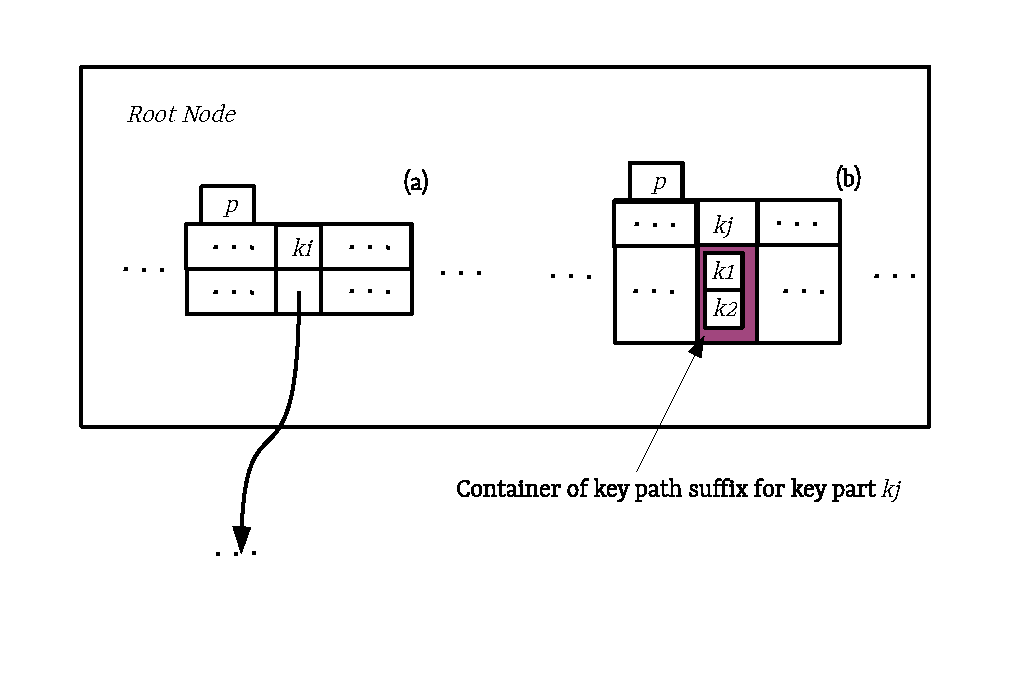
\includegraphics{figures/chapter4/depth3}
	\caption{Depth 3 Node}
	\label{fig:compressed_depth_3_node}
\end{figure}

\begin{figure}
	\centering
	\vspace{-1in}
	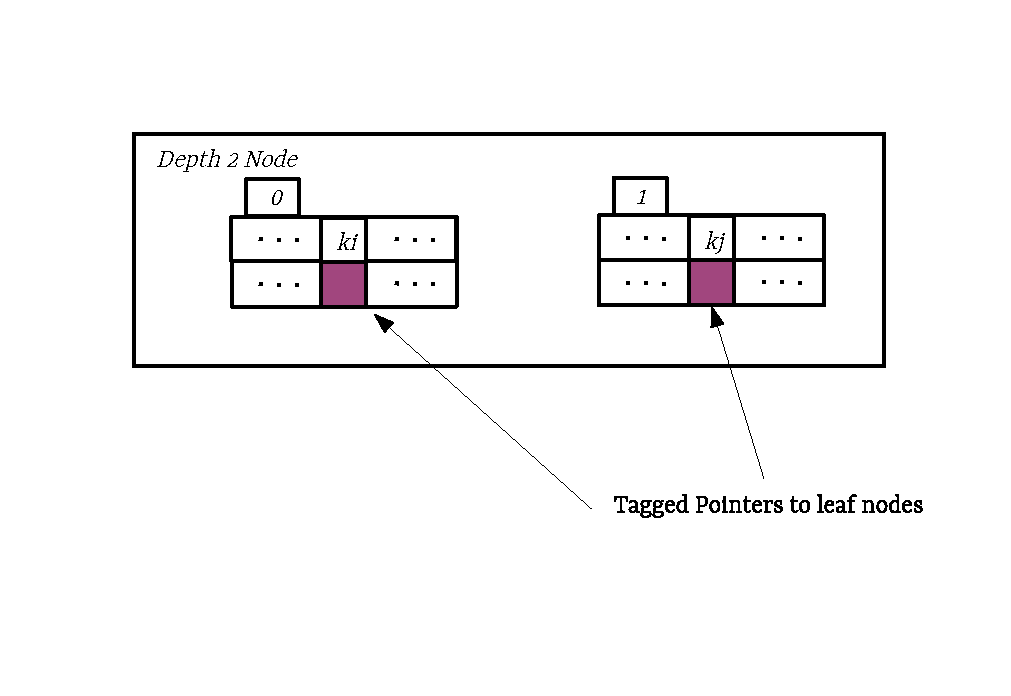
\includegraphics{figures/chapter4/depth2}
	\caption{Depth 2 Node}
	\label{fig:compressed_depth_2_node}
\end{figure}
\clearpage

\subsection{Virtual Nodes}
Due to the fact that some key paths in Hypertrie are collapsed into a single node of depth $d$, we still need to maintain the concept that collapsed path still represents a tensor of the order $d-1$ with a single entry that evaluates to 1. Maintaining the concept becomes very important when we implement Hypertrie programmatically. In particular, when we want to perform slicing in the position of the collapsed path. \\

A straight forward solution is to return the container representation of the collapsed path (array, int value) from the slicing call. However, that contradicts with slicing function contract defined in the Hypertrie interface which states that slicing always return a child node. Also, following this approach will add extra code complexity in the context of handling the different types of returned values from slicing. It will also force us to define a different behavior for each returned type from slicing resulting in substantial amount of code redundancy.  \\

A clean solution is to encapsulate the defined key path containers in a special type of Hypertrie nodes. 
Those nodes realize all the methods defined in the Hypertrie interface. 
As a result, we treat slicing operations uniformally. 
I call these wrappers \textbf{virtual nodes} to discriminate them from the actual Hypertrie nodes which I call \textbf{concrete nodes}. \\

Back to the previous sub section \ref{ch:approach_node_structure}, I defined two types of key chain static containers. 
Concretely, a static array of length 2 representing the key suffix of compressed edges in the root node. 
A tagged pointer that bounds the key suffix (a single key part) of compressed edges in internal depth 2 nodes. 
Hence, we now have two variants of nodes for each depth (except for the root node). Concrete nodes and virtual nodes. \\

In the original Hypertrie implementation, slicing method gives enough information about the child node being returned from its execution as shown in listing \ref{lst:slicing_original_hypertrie}. 
As we conceptually expanded the set of Hypertrie nodes to include virtual nodes, the pointer to a child node of a certain depth returned from a slicing must carry information about the nature of the node being concrete or virtual.

\begin{lstlisting}[caption={Slicing method signituar defined for node where d = $depth$ in original Hypertrie},label={lst:slicing_original_hypertrie},language=C++]
#include <array>

template<int depth>
class hypertrie_node {
	....
	template<typename key_part_type>
	using SliceKey = std::array<std::optional<key_part_type>, depth>;
	....
	template<int slice_depth>
	hypertrie_node<slice_count>* slice(SliceKey slice_key) {
		....
	}
	....
}
\end{lstlisting} 

To accomplish this, we again use tagged pointers. This time, the pointer holds only a memory address of type \texttt{void *}. However, the tag here is used to distinguish between the referenced node being concrete or virtual. Accordingly, we can cast the the pointer value to the appropriate type based on the tag value. 
It becomes the responsibility of the slicing method to create and return that pointer properly. Listing \ref{lst:node_tagged_pointer} shows the structure of the tagged pointer I developed to reference different node types in our space-friendly Hypertrie. 

\begin{lstlisting}[caption={Node pointer structure},label={lst:node_tagged_pointer},language=C++]

template<typename VirtualNodePtr, typename ConcreteNodePtr, int alignedTo>
class NodePointer {
	private:
	  	static const intptr_t tagMask = alignedTo - 1;
	    static const intptr_t pointerMask = ~tagMask;
	  
	public:
		static constexpr int VIRTUAL = 1;
		
		static constexpr int CONCRETE = 0;
	
	protected:
		union {
		  	void *asPointer;
		  	uintptr_t asBits;
		}
      
	public:
        inline NodePointer(VirtualNodePtr ptr) {
	        // Safer to clear the tag as we set a fresh tag in the setter method
	        clearTag();
	        asPointer = ptr;
	        asBits |= VIRTUAL;
        }
        
        inline void clearTag() {
       		asBits &= pointerMask;
        }
        
		inline NodePointer(ConcreteNodePtr ptr) {
        	clearTag();
           	asPointer = node;
           	asBits |= CONCRETE;
        }
        
        /**
        * @param ptr it is already a tagged pointer
        */
        inline NodePointer(void *ptr) {
	       	asPointer = ptr;
        }
        
        inline NodePointer() {
        	asPointer = nullptr;
        }
}
\end{lstlisting} 

\begin{lstlisting}[caption={Slicing method signituar defined for node where d = $depth$ in the space-friendly Hypertrie},label={lst:slicing_original_hypertrie},language=C++]
#include <array>

template<int depth, bool virtual>
class hypertrie_node {
  ...
  template<typename key_part_type>
  using SliceKey = std::array<std::optional<key_part_type>, depth>;
  ....
  template<int depth>
  using NodePointer = 
    TaggedPointer<hypertrie_node<depth, false>, hypertrie_node<depth, true>>;
  ....
  template<int slice_depth>
  NodePointer<slice_depth> slice(SliceKey slice_key) {
 	....
  }
  ....
}
\end{lstlisting} 



\section{Algorithms}
The change in the internal nodes representations in the compressed version of Hypertrie leads to change in how we define its behavior. 
Hence, the new realization add the logic necessary to consider the compressed paths containers. 
At the same time, the logic has to have the same contract defined in the original Hypertrie interface. 
Following that approach will allow us to integrate the new Hypertrie implementation into the Tentris system efficiently. \\

Next, I list the main algorithms that realize the core behaviors of Hypertrie when the space reduction approach is applied. The great proportion of my work was on expanding the code base of Hypertrie project to adapt the key path compression approach including the implementation of the accompanying algorithms\footnote{In this section, I list only the main algorithms}.

\subsection{Key Retrieval}
A basic operation in Hypertrie is to check if a given key $k \in N^d$ represents a path from a hypertrie node $h \in H(d)$ to a leaf node. Due to the presence of key path containers in internal nodes, the logic should be expanded to consider the children paths of both the compressed and non-compressed edges in each node type. \\

\paragraph{depth 3 Node}

\paragraph{depth 2 Node}

\paragraph{depth 1 Node}

\begin{algorithm}
	\DontPrintSemicolon
	\SetAlgoLined
	\KwIn{$node3$: a depth 3 node, $depth$: current node depth, $key$: array of key parts $k_{i} \in K_{i}$ of size 3}
	\KwOut{a boolean if a key represents a path in Hypertrie}
	\SetKwFunction{KwFn}{node3\_key\_retrieval}
    \KwFn{node3, depth, key} \;
    \Begin{
    	$p_{min} \gets\;$\texttt{minCardPos(}$node3$\texttt{)} \;
    	$k_{i} \gets key[p_{min}]$ \;
    	
		$arr_{i} \gets HTComm_{p_{min}}[k_{i}]$\;
		\If{$arr_{i}\;!=NULL$}{
			$l \gets 0$ \;
			$c \gets 0$ \;
			\While{$l < depth$}{
				\eIf{$l\;==\; p_{min}$}{
					$l = l + 1$\;
				}{
					\If{$arr_{i}[c]\; != \;key[l]$}{
						\textbf{return} $false$\;
					}
					$l = l + 1$ \;
					$c = c + 1$ \;
				}
			}
			\textbf{return} $true$\;
		}
		$child_{i} \gets HT_{p_{min}}[k_{i}]$\;
		\eIf{$child_{i}\;!=\; NULL$}{
			$subkey \gets <0,0>$\;
			$l \gets 0$ \;
			$c \gets 0$ \;
			\While{$l < depth$}{
				\eIf{$l\;==\; p_{min}$}{
					$l = l + 1$\;
				}{
					$subkey[c] \gets key[l]$\;
					$l = l + 1$ \;
					$c = c + 1$ \;
				}
			}
			\textbf{return} \texttt{node2\_key\_retrieval(}$child_{i}, 2, subkey$\texttt{)}\;
		}{
			\textbf{return} $false$\;
		}
	}
\caption{\sc Key Retrieval in the root node}
\label{algo:key_retrieval_depth3}

\end{algorithm}


\begin{algorithm}
	\DontPrintSemicolon
	\SetAlgoLined
	\KwIn{$node2$: a depth 2 node\\
		$depth$: current node depth\\
		$key$: array of key parts $k_{i} \in K_{i}$ of size 2 representing a sub key}
	\KwOut{a boolean if a key represents a path in Hypertrie}
	\SetKwFunction{KwFn}{node2\_key\_retrieval}
	\KwFn{node2, depth, key} \;
	\Begin{
		$p_{min} \gets\;$\texttt{minCardPos(}$node3$\texttt{)} \;
		$k_{i} \gets key[p_{min}]$ \;
		$ptr_{i} \gets HT{p_{min}}[k_{i}]$\;
		\lIf{$ptr_{i}\; ==\; NULL$}{\textbf{return} false}
		$(value_{i}, tag_{i}) \gets ptr_{i}$ \;
		$next\_pos \gets (p_{min} + 1) \;\% \;2$\;
		\eIf{$tag_{i} == INT\_TAG$}{
	    	\textbf{return} $value_{i} == key[next\_pos] $
		}{
			$subkey \gets <key[next\_pos]>$\;
			$child_{i} \gets $ \texttt{getPointer(}$value_{i}$\texttt{)}\;
			\textbf{return} \texttt{node1\_key\_retrieval(}$child_{i}, 1, subkey$\texttt{)}\;
	    }
	}
	\caption{\sc Key Retrieval in depth 2 Nodes}
	\label{algo:key_retrieval_depth2}
	
\end{algorithm}

\begin{algorithm}
	\DontPrintSemicolon
	\SetAlgoLined
	\KwIn{$node1$: a depth 1 node\\
		$depth$: current node depth\\
		$key$: array of key parts $k_{i} \in K_{i}$ of size 2 representing a sub key}
	\KwOut{a boolean if a key represents a path in Hypertrie}
	\SetKwFunction{KwFn}{node1\_key\_retrieval}
	\KwFn{node1, depth, key} \;
	\Begin{
		\textbf{return} set of edges in $node1$ holds the key part $key[0]$\;
	}
	\caption{\sc Key Retrieval in depth 1 Nodes}
	\label{algo:key_retrieval_depth1}
	
\end{algorithm}

\clearpage

\subsection{Key Insertion} 
Similar to other tree-based data structures, the key insertion operation is recursive. Due to the fact that nodes at certain depth enjoys a unique  internal structure, the algorithm for adding keys will change depending on the target node in the recursion sequence. To achieve key insertion, two auxiliary constructs must be implemented. First, the algorithm should utilize a mechanism that keeps track of the processed key parts so far for each key path in hypertrie. A way to maintain such state information is to use a tuple $processed \in \mathbb{B}^3$, such that:\\

\centerline{$\forall i \in \mathbb{N}_3 , processed[i] = \left\{ \begin{array}{rc} 1, & \mbox{key part at position }i\mbox{ is processed} \\ 0,  & \mbox{otherwise} \\ \end{array} \right.$}

\hspace{2cm}

Utilizing the state tuple $processed$ while processing a hypertrie node, we know the \textit{sub key}, the remaining key parts to be added. Hence, the state tuple is updated as we proceed in the construction of the key path during insertion; i.e. processing more key parts. \\

 For that, a couple of utility functions are used to map the main key to sub keys. That is, they map key part indices of the inserted key to dimensions represented by the succeeding child node and vise versa. By that, we know which key part should be inserted at which position. $pos2ids$ maps node positions to key part indices, and $id2pos$ maps key part indices to node positions. Both functions are defined in the following:\\
 
 \centerline{$pos2id(pos, processed) = pos + |\{e | e \in$ dom($processed$)$, e \leq pos, processed[e] = 1\}|$}
 \hspace{2cm}
 
 \centerline{$id2pos(id, processed) = id - |\{e | e \in$ dom($processed$)$, e \leq id, processed[e] = 1\}|$}
 \hspace{2cm}
 
 The second requirement to achieve efficient insertion similar to the original hypertrie insertion method is to preserve the concept of pointing to equal child nodes only once. This is done by setting up a dictionary $processed\_nodes: \mathbb{B}^3 \to node$ for each key insertion call.  $processed\_nodes$ maps instances of the state tuple $processed$ to inform which hypertrie nodes were already created for which combination of dimensions.

\begin{algorithm}
	\DontPrintSemicolon
	\SetAlgoLined
	\KwIn{$node3$: a depth 3 node, $depth$: current node depth, $key$: array of key parts}
	\SetKwFunction{KwFn}{insert}
	\KwFn{node3, depth, key} \;
	\Begin{
		$processed \gets <0,0,0>$\;
		$processed\_nodes \gets \{\}$\;
		\texttt{node3\_insert(}$node3, depth, key, processed, processed\_nodes$\texttt{)}
	}
	\caption{\sc Key insertion main method}
	\label{algo:key_insert}
\end{algorithm}
\clearpage
\begin{algorithm}
	\DontPrintSemicolon
	\SetAlgoLined
	\KwIn{$node3$: a depth 3 node, $depth$: current node depth, $key$: array of key parts,\\ $processed$: state of processed key parts, $processed\_nodes$: dictionary of processed nodes}
	\SetKwFunction{KwFn}{node3\_insert}
	\KwFn{node3, depth, key, processed, processed\_nodes} \;
	\Begin{
		\ForEach{$key\_pos$ in $\{e | e \in$ dom($processed$)$, processed[e] = 0\}$}{
			$key\_part \gets key[key\_pos]$\;
			$pos \gets id2pos(key\_pos, processed)$\;
			$next\_processed = processed$ \;
			$next\_processed[key\_pos] \gets1$ \;
			$child\_ptr \gets$ \texttt{get(}$node3, pos, key\_part$\texttt{)}\;
			$(child, tag) \gets child\_ptr$\;
			\uIf{$child$ is empty}{
				$arr \gets [0, 0]$\;
				\For{$i$ in $[0, 1]$}{
					$arr[i] = key[pos2id(i, next\_processed)]$\;
				}
				$HTComm_{pos}[key\_part] = arr$\;
			}\uElseIf{$tag == NON\_COMPRESSED$}{
				\texttt{node2\_insert(}$child, 2, key, next\_processed, processed\_nodes$\texttt{)}\;
			}
			\ElseIf{$tag == COMPRESSED$}{
				$new\_node \gets$ create a new concrete hypertrie child node of depth 2\;
				$HT_{pos}[key\_part] = ptr(new\_node)$\;
				\texttt{node2\_insert(}$new\_node, 2, key, next\_processed, processed\_nodes$\texttt{)}\;
				$reconstruced\_key \gets <0, 0, 0>$\;
				$arr \gets HTComm_{pos}[key\_part]$\;
				\For{$i$ in $[0, 1, 2]$}{
					\uIf{$i == key\_pos$}{
						$reconstruced\_key[i] = key\_part$\;
					}
					\Else{
						$reconstruced\_key[i] = arr[id2pos(i,next\_processed)]$\;
					}
				}
				erase $HTComm_{pos}[key\_part]$\;
				\texttt{node2\_insert(}$new\_node, 2, reconstruced\_key, next\_processed,processed\_nodes$\texttt{)}\;
			}
		}
	}
	\caption{\sc Key insertion for depth 3 node}
	\label{algo:key_insert_node3}
\end{algorithm}


\begin{algorithm}
	\DontPrintSemicolon
	\SetAlgoLined
	\KwIn{$node2$: a depth 2 node, $depth$: current node depth, $key$: array of key parts,\\ $processed$: state of processed key parts, $processed\_nodes$: dictionary of processed nodes}
	\SetKwFunction{KwFn}{node2\_insert}
	\KwFn{node2, depth, key, processed, processed\_nodes} \;
	\Begin{
		$processed\_nodes[processed] \gets node2$ \;
		\ForEach{$key\_pos$ in $\{e | e \in$ dom($processed$)$, processed[e] = 0\}$}{
			$key\_part \gets key[key\_pos]$\;
			$pos \gets id2pos(key\_pos, processed)$\;
			$next\_processed \gets$ cloning $processed$\;
			$next\_processed[key\_pos] \gets 1$ \;
			$child\_ptr \gets HT{pos}[key\_part]$\;
			$(value, tag) \gets child\_ptr$\;
			\uIf{$child\_ptr$ is empty}{
				$next\_key\_part = key[pos2id(0, next\_processed)]$\;
				$HT_{pos}[key\_part] \gets$ tagged pointer holding $next\_key\_part$ integer\;
			}\Else{
				\uIf{$tag = IS\_POINTER$}{
					$child\_node \gets$ node to which address in $value$ points\;
					\texttt{node1\_insert(}$child\_node, 1, key, next\_processed,processed\_nodes$\texttt{)}\;
				}\ElseIf{$tag = IS\_INT$}{
					$created\_node \gets processed\_nodes[next\_processed]$\;
					\uIf{$created\_node$ exists}{
						$value \gets$ hold a pointer to $created\_node$ \;
						$tag \gets IS\_POINITER$ \;
					}\Else{
						$reconstruced\_key \gets <0, 0, 0>$\;
						\For{$i$ in $[0, 1, 2]$}{
							\lIf{$processed[i] == 1$}{$reconstruced\_key[i] = key[i]$}
							\lElseIf{$i == key\_pos$}{$reconstruced\_key[i] = key\_part$}
							\lElse{$reconstruced\_key[i] = value$}
						}
					}
					$new\_node \gets$ create a new concrete hypertrie child node of depth 1\;
					$HT_{pos}[key\_part] \gets$ tagged pointer holding pointer to $new\_child$\;
					\texttt{node1\_insert(}$new\_node, 1, key, reconstruced\_key,next\_processed,processed\_nodes$\texttt{)}\;
				}
			}
		}
	}
	\caption{\sc Key insertion for depth 2 node}
	\label{algo:key_insert_node2}
\end{algorithm}


\begin{algorithm}[h]
	\DontPrintSemicolon
	\SetAlgoLined
	\KwIn{$node1$: a depth 1 node, $depth$: current node depth, $key$: array of key parts,\\ $processed$: state of processed key parts, $processed\_nodes$: dictionary of processed nodes}
	\SetKwFunction{KwFn}{node1\_insert}
	\KwFn{node1, depth, key, processed, processed\_nodes} \;
	\Begin{
		$created\_node \gets processed\_nodes[processed]$\;
		\If{$created\_node$ does not exist}{
			$processed\_nodes[processed] = node1$\;
		}
		$key\_part \gets key[pos2id(0, processed)]$\;
		add $key\_part$ to the set of key parts (edges) held by $node1$\;
	}
	\caption{\sc Key insertion for depth 1 node}
	\label{algo:key_insert_node1_single_key}
\end{algorithm}

\begin{algorithm}[h]
	\DontPrintSemicolon
	\SetAlgoLined
	\KwIn{$node1$: a depth 1 node, $depth$: current node depth, $key, reconstruced\_key$: array of key parts,\\ $processed$: state of processed key parts, $processed\_nodes$: dictionary of processed nodes}
	\SetKwFunction{KwFn}{node1\_insert}
	\KwFn{node1, depth, key, processed, reconstruced\_key, processed\_nodes} \;
	\Begin{
		$created\_node \gets processed\_nodes[processed]$\;
		\lIf{$created\_node$ does not exist}{
			$processed\_nodes[processed] = node1$\;
		}
		$key\_part_{1} \gets key[pos2id(0, processed)]$\;
		$key\_part_{2} \gets reconstruced\_key[pos2id(0, processed)]$\;
		add $key\_part$ and $key\_part_{2}$ to the set of key parts (edges) held by $node1$\;
	}
	\caption{\sc Key insertion for depth 1 node including the insertion of the reconstructed key}
	\label{algo:key_insert_node1_double_key}
\end{algorithm}

\clearpage
